\documentclass{article}
\usepackage{titlesec}
\usepackage{mhchem}
\usepackage{array}
\usepackage{graphicx}
\usepackage[bmargin=2cm, tmargin=2cm]{geometry}
\usepackage{fourier-orns}

\newcommand{\thedate}[1]{\hfill{\small\sc #1}}
\newcommand{\NB}{{\large\lefthand}\quad}
\newcommand{\cm}{cm\(^{-1}\) }
\titleformat{\section}[hang]{\sc\Large}{\S\thesection}{3ex}{}[]
\titleformat{\subsection}[runin]{\sc\large}{\S\thesubsection}{3ex}{}[]
\titleformat{\subsubsection}[runin]{}{\S\thesubsubsection}{1ex}{\bfseries}[.]

\newtheorem{defn}{Definition}[section]

\title{Energy, Spectroscopy and Solid State Chemistry}
\date{}
\author{}
\begin{document}
    \maketitle
    \section{Spectroscopy}
    \subsection{Introduction}\thedate{28/10/20 --- Week 1}
    \subsubsection{The Born-Oppenheimer Approximation}
    The assumption that the electronic motion and the nuclear motion in molecules can be separated, due to the
    difference in mass between the electron and the nuclei.
    \begin{align*}
        \Psi_{tot} &= \psi_{el} \psi_{nuc}\\
        \text{Where the resulting total} & \text{ energy is a simple sum.}\\
        E_{tot} &= E_{el} + E_{nuc}
    \end{align*}
    It is very convinient, although slightly less rigorous, to factorise \(\Psi_{nuc}\) into vibrational and
    rotational parts. Translational energy is unquantised and so useless for spectroscopy.
    \begin{align*}
        \Psi_{tot} &= \psi_{el} \psi_{vib} \psi_{rot}\\
        E_{tot} &= E_{el} + E_{vib} + E_{rot}
    \end{align*}
    \begin{figure}[h]
        \centering
        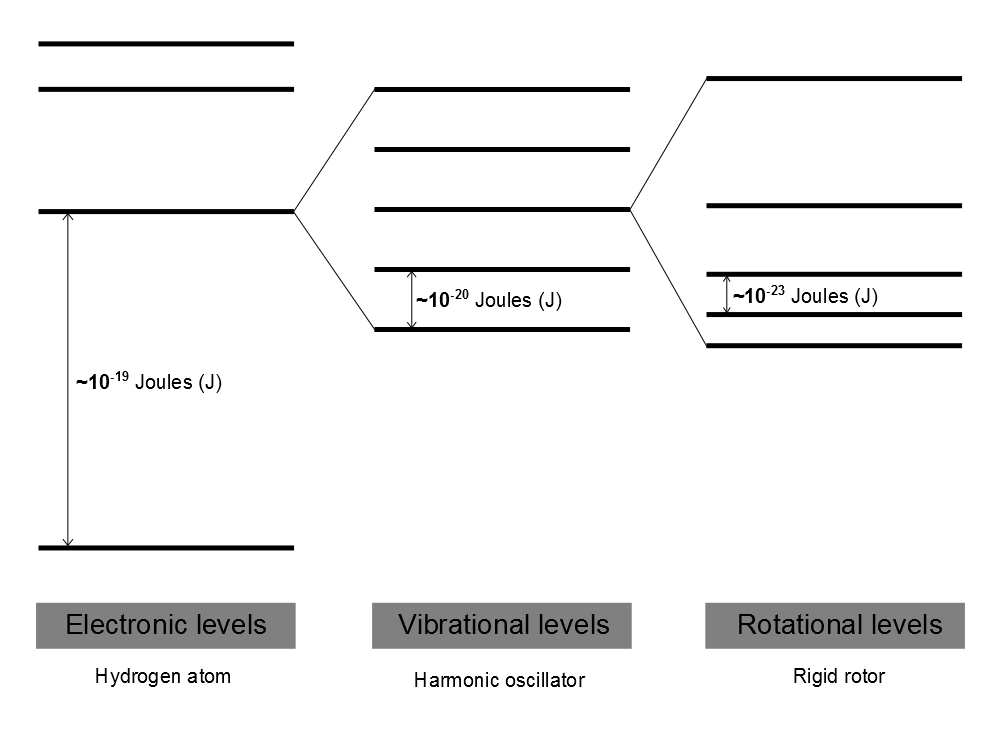
\includegraphics[width=10cm]{trans.png}
        \caption{Transitions of different energy levels}
    \end{figure}

    \begin{tabular}[2cm]{l l l l}
        \(\Delta \text{E} \approx \) \hspace{1cm}  & \(10^{4} - 10^{5} \text{cm}^{-1}\) \hspace{0.8cm} & \(10^{2} - 10^{3} \text{cm}^{-1}\) \hspace{0.8cm} & \(0.1 - 10 \text{cm}^{-1}\)\\
        Transitions at \(\Delta \lambda \approx \) & \(500 - 100 \text{nm}\) \hspace{0.5cm} & \(100 - 2 \mu \text{m} \) \hspace{0.5cm} & \(10 \text{cm} - 1 \text{mm}\)\\
        Light range & Vis-UV & Infrared & Microwave\\
    \end{tabular}

    \vspace{1cm}
    Every electronic energy level contains multiple vibrational levels which contains multiple rotational levels.
    More on this to come. 

    \subsubsection{The Boltzmann Law} At thermal equilibrium the relativep population of the \(i^{\text{th}}\) energy level is given by:
    \begin{align*}
        \frac{n_i}{n_0} = \frac{g_i}{g_0}e^{-\frac{\Delta E_i}{k_B T}}
    \end{align*}
    \begin{itemize}
        \item \(g_i\) is the degeneracy of the \(i\)th level (the number of states with the same energy)
        \item \(\Delta E_i\) is the energy difference between the lowest (ground) and \(i\)th levels
        \item \(k_B\) is the Boltzmann constant
        \item $T$ is the temperature (in Kelvin, obviously)
    \end{itemize}

    Ezxcffample: FGind the relative populations of the lowest two energy levels for each in a CO molecule at 298k if
    \begin{enumerate}
        \item The two lowest rotational levels are 3.382 cm$^{-1}$ apart with $g_1$ = 3 and $g_0$ = 1
        \item The two lowest vibrational levels are 1743 cm$^{-1}$ apart each with a degeneracy of 1
        \item The two lowest electronic levels are 48690 cm$^{-1}$ apart with $g_1$ = 6 and $g_0$ = 1
    \end{enumerate}

    Since we are given the energy spacings in cm\(^{-1}\) we should convert our $k_BT$ to cm$^{-1}$ by using
    \(\frac{E}{hc} = \nu\) so $k_BT$ = 207\cm. From here the calculations are relatively simple.
    \begin{enumerate}
        \item \(\frac{3}{1}e^{-\frac{3.382}{207}} = 2.95\)
        \item \(\frac{1}{1}e^{-\frac{1743}{207}} = 2.24\text{x}10^{-4}\)
        \item \(\frac{6}{1}e^{-\frac{48690}{207}} = 4.2\text{x}10^{-102} \text{ so small it might as well be 0}\)
    \end{enumerate}

    What does this tell us? At normal temperatures there is enough energy to promote to higher rotational 
    energy levels. Since $k_BT$ = 207\cm and rotational levels are separated by only 10\cm this should be obvious.
    It is also clear that there is nowhere near enough energy at normal temperatures for there to much vibrational
    tranistion, and not enough energy for there to be any electronic tranistions at all.
\end{document}